% !TeX root = RJwrapper.tex
\title{gdpR: An R Package for studying differentially private algorithms}


\author{by Jordan A. Awan, Kevin Eng, Robin Gong, Nianqiao Phyllis Ju, and Vinayak A. Rao}

\maketitle

\abstract{%
This paper serves as a reference and introduction on using the \(gdpR\) R package. The goal of this package is to provide some tools for exploring the impact of different privacy regimes on a Bayesian analysis. A strength of this framework is the ability to target the exact posterior in settings where the likelihood is too complex to analytically express.
}

\hypertarget{introduction}{%
\section{Introduction}\label{introduction}}

The ease and pervasiveness of modern data collection technologies has raised
concerns about data privacy. (Dwork and Roth 2013) introduced the differential privacy
framework as a means to rigorously define privacy. The framework has lead to the
development of many ``privitized'\,' versions of existing statistical methods. The
process of privitizing usually consist of introducing random noise in someway using
a known distribution.

\hypertarget{overview-of-the-gdpr-packge}{%
\section{overview of the gdpR packge}\label{overview-of-the-gdpr-packge}}

This section reviews This will show a verbatim inline R expression \texttt{\textasciigrave{}r\ 1+1\textasciigrave{}} in the output.

\hypertarget{background}{%
\section{Background}\label{background}}

Some packages on interactive graphics include \CRANpkg{plotly} (Sievert 2020) that interfaces with Javascript for web-based interactive graphics, \CRANpkg{crosstalk} (Cheng and Sievert 2021) that specializes cross-linking elements across individual graphics. The recent R Journal paper \CRANpkg{tsibbletalk} (Wang and Cook 2021) provides a good example of including interactive graphics into an article for the journal. It has both a set of linked plots, and also an animated gif example, illustrating linking between time series plots and feature summaries.

\hypertarget{customizing-tooltip-design-with}{%
\section{\texorpdfstring{Customizing tooltip design with \pkg{ToOoOlTiPs}}{Customizing tooltip design with }}\label{customizing-tooltip-design-with}}

\pkg{ToOoOlTiPs} is a packages for customizing tooltips in interactive graphics, it features these possibilities.

\hypertarget{a-gallery-of-tooltips-examples}{%
\section{A gallery of tooltips examples}\label{a-gallery-of-tooltips-examples}}

The \CRANpkg{palmerpenguins} data (Horst, Hill, and Gorman 2020) features three penguin species which has a lovely illustration by Alison Horst in Figure \ref{fig:penguins-alison}.

\begin{figure}
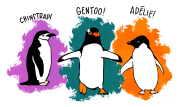
\includegraphics[width=1\linewidth,height=0.3\textheight]{figures/penguins} \caption{Artwork by \@allison\_horst}\label{fig:penguins-alison}
\end{figure}

Table \ref{tab:penguins-tab-static} prints at the first few rows of the \texttt{penguins} data:

\begin{table}

\caption{\label{tab:penguins-tab-static}A basic table}
\centering
\fontsize{7}{9}\selectfont
\begin{tabular}[t]{l|l|r|r|r|r|l|r}
\hline
species & island & bill\_length\_mm & bill\_depth\_mm & flipper\_length\_mm & body\_mass\_g & sex & year\\
\hline
Adelie & Torgersen & 39.1 & 18.7 & 181 & 3750 & male & 2007\\
\hline
Adelie & Torgersen & 39.5 & 17.4 & 186 & 3800 & female & 2007\\
\hline
Adelie & Torgersen & 40.3 & 18.0 & 195 & 3250 & female & 2007\\
\hline
Adelie & Torgersen & NA & NA & NA & NA & NA & 2007\\
\hline
Adelie & Torgersen & 36.7 & 19.3 & 193 & 3450 & female & 2007\\
\hline
Adelie & Torgersen & 39.3 & 20.6 & 190 & 3650 & male & 2007\\
\hline
\end{tabular}
\end{table}

Figure \ref{fig:penguins-ggplot} shows an plot of the penguins data, made using the \CRANpkg{ggplot2} package.

\begin{verbatim}
penguins %>% 
  ggplot(aes(x = bill_depth_mm, y = bill_length_mm, 
             color = species)) + 
  geom_point()
\end{verbatim}

\begin{figure}
\centering
\includegraphics{dppaper_files/figure-latex/penguins-ggplot-1.pdf}
\caption{\label{fig:penguins-ggplot}A basic non-interactive plot made with the ggplot2 package on palmer penguin data. Three species of penguins are plotted with bill depth on the x-axis and bill length on the y-axis. Visit the online article to access the interactive version made with the plotly package.}
\end{figure}

\hypertarget{summary}{%
\section{Summary}\label{summary}}

We have displayed various tooltips that are available in the package \pkg{ToOoOlTiPs}.

\hypertarget{references}{%
\section*{References}\label{references}}
\addcontentsline{toc}{section}{References}

\hypertarget{refs}{}
\begin{CSLReferences}{1}{0}
\leavevmode\vadjust pre{\hypertarget{ref-crosstalk}{}}%
Cheng, Joe, and Carson Sievert. 2021. \emph{{crosstalk}: Inter-Widget Interactivity for HTML Widgets}. \url{https://CRAN.R-project.org/package=crosstalk}.

\leavevmode\vadjust pre{\hypertarget{ref-Dwork2013}{}}%
Dwork, Cynthia, and Aaron Roth. 2013. {``The Algorithmic Foundations of Differential Privacy.''} \emph{Foundations and Trends{\textregistered} in Theoretical Computer Science} 9 (3-4): 211--407. \url{https://doi.org/10.1561/0400000042}.

\leavevmode\vadjust pre{\hypertarget{ref-palmerpenguins}{}}%
Horst, Allison Marie, Alison Presmanes Hill, and Kristen B Gorman. 2020. \emph{{palmerpenguins}: Palmer Archipelago (Antarctica) Penguin Data}. \url{https://allisonhorst.github.io/palmerpenguins/}.

\leavevmode\vadjust pre{\hypertarget{ref-plotly}{}}%
Sievert, Carson. 2020. \emph{{Interactive Web-Based Data Visualizatio}n with r, Plotly, and Shiny}. Chapman; Hall/CRC. \url{https://plotly-r.com}.

\leavevmode\vadjust pre{\hypertarget{ref-RJ-2021-050}{}}%
Wang, Earo, and Dianne Cook. 2021. {``Conversations in Time: Interactive Visualisation to Explore Structured Temporal Data.''} \emph{The R Journal}. \url{https://doi.org/10.32614/RJ-2021-050}.

\end{CSLReferences}

\bibliography{RJreferences.bib}

\address{%
Jordan A. Awan\\
Purdue University\\%
Department of Statistics\\ West Lafayette, IN 47907\\
%
\url{https://www.britannica.com/animal/quokka}\\%
%
\href{mailto:jawan@purdue.edu}{\nolinkurl{jawan@purdue.edu}}%
}

\address{%
Kevin Eng\\
Rutgers University\\%
Department of Statistics\\ Piscataway, NJ 08854\\
%
\url{https://www.britannica.com/animal/quokka}\\%
%
\href{mailto:ke157@stat.rutgers.edu}{\nolinkurl{ke157@stat.rutgers.edu}}%
}

\address{%
Robin Gong\\
Rutgers University\\%
Department of Statistics\\ Piscataway, NJ 08854\\
%
\url{https://www.britannica.com/animal/quokka}\\%
%
\href{mailto:ruobin.gong@rutgers.edu}{\nolinkurl{ruobin.gong@rutgers.edu}}%
}

\address{%
Nianqiao Phyllis Ju\\
Purdue University\\%
Department of Statistics\\ West Lafayette, IN 47907\\
%
\url{https://www.britannica.com/animal/quokka}\\%
%
\href{mailto:nianqiao@purdue.edu}{\nolinkurl{nianqiao@purdue.edu}}%
}

\address{%
Vinayak A. Rao\\
Purdue University\\%
Department of Statistics\\ West Lafayette, IN 47907\\
%
\url{https://www.britannica.com/animal/quokka}\\%
%
\href{mailto:varao@purdue.edu}{\nolinkurl{varao@purdue.edu}}%
}
